\documentclass[a4paper,12pt]{article}
%改变页边距
\usepackage[english]{babel}
\usepackage{geometry}
\geometry{left=1.5cm,right=1.5cm,top=2.0cm,bottom=2cm}
\usepackage{latexsym}
\usepackage{amsmath}
\usepackage{times}
\usepackage{graphicx}
\usepackage{epstopdf}
\usepackage{booktabs}
\usepackage{float}
\usepackage[numbers]{natbib}
\citestyle{IEEE}
\usepackage{subfigure}
\usepackage{indentfirst} % 段首空格
%\usepackage[utf8]{inputenc}
%\usepackage[english]{babel}
\usepackage{gensymb}
\newtheorem{theorem}{Theorem}[section]
\newtheorem{corollary}{Corollary}[theorem]
\newtheorem{lemma}[theorem]{Lemma}
\usepackage{ gensymb }
\usepackage{indentfirst} 
\usepackage{times}
\begin{document}
	\title{Homework 1}
	\author{
			Wenting LI
		\and
			liw14@rpi.edu
			}
	\maketitle


 \section*{1. }
\subsection*{a. }
Given a $(\Delta+1)$-colorable graph, where $\Delta$ is the maximum degree of any vertex in $G=(V,E)$,

\begin{enumerate}
\item[1. ]Find the vertex $v$ in $G$ with the maximum degree $\Delta$ and its neighbor $N(v)=\{w | (v,w) \in E, i=1,\dots,\Delta \}$;

\item[2. ]First color $v$ with one color, then color its neighbors $w_i \in N(v)$ one by one. If $w_i$ is also connected to $w_j, i\neq j$, then color them with different colors. In this way, we need at most $\Delta +1$ colors to color $v$ and its neighbor  $N(v)$;

\item[3. ]Then find another $v^{\prime}$ not colored yet and its neighbor $N(v^{\prime})=\{w | (v^{\prime},w) \in E, i\leq \Delta \}$. Color them in the same way as step (2) using the $\Delta +1$ colors;

\item[4. ]Continue to color all other vertexes with less than $\Delta +1$ colors until the graph $G$ is completely colored.
\end{enumerate}

As we can color G in poly-time with at most $(\Delta +1)$ colors, then $G$ is $(\Delta +1)$ colorable.
\subsection*{b. }
Bipartite graph is an undirected graph with nodes partitioned into group $X$ and $Y$. For each line, its one ending node is in group $X$ and the other ending node is in $Y$. 

Then we can color all the nodes in group $X$ with one color and the nodes in group $Y$ with the other color. Therefore, bipartite graphs are $2$-colorable. 

\subsection*{c.}
Given undirected 3-colorable graph $G=(V,E)$,  $|V|=n$.
For each $v \in V$ vertext, let $d(v)$ be the degree of $v$.

If $d(v)\geq \sqrt{(n)}$, then remove $v$ and its neighbors $N(v)=\{w_i| (v,w_i) \in E, i\geq \sqrt{(n)}\}$, and color $v$ with the first color and then color its neighbor $w_1$ with the second color, and then color all other neighbors one by one. If two of its neighbors $w_i, w_j$ are connected, then color them with the second and the third color, otherwise color the neighbors with the second color. We can color the subgraph with a poly-time $O(n)$.

As graph $G$ is a 3 colorable graph and thus its subgraph is also a 3-colorable graph, thus we need at most 3 colors to color each subgraph. 

Each time we remove at most $\sqrt{n}+1$ vetex from $G$, which has $n$ vertex in total, thus we need to remove at most $ \sqrt{(n)} $. As we need color each subgraph with at most 3 colors, then in order to color all these vertex and its neighbors, we need at most $O(\sqrt{n})$ colors. 

Until all the vertex in $G$ have degree less than $\sqrt{(n)}$, we can apply the algorithm in (a) to color them with $O(\sqrt{(n)})$ colors with a poly-time.

In summary, we need $O(\sqrt{n}) $ colors.
\subsection*{d.}
Given undirected 3-colorable graph $G=(V,E)$,  $|V|=n$.
For each $v \in V$ vertext, let $d(v)$ be the degree of $v$.\\
If $d(v)\geq n^{\frac{2}{3}}$, then remove $v$ and its neighbors $N(v)=\{w_i| (v,w_i) \in E, i\geq \sqrt{(n)}\}$, and color $v$ with the first color and then color its neighbor $w_1$ with the second color, and then color all other neighbors one by one. If two of its neighbors $w_i, w_j$ are connected, then color them with the second and the third color, otherwise color the neighbors with the second color. We can color the subgraph with a poly-time $O(n)$.

As graph $G$ is a 4 colorable graph and thus its subgraph is also a 3-colorable graph, thus we need at most 4 colors to color each subgraph. 

Each time we remove at most $(n^{\frac{2}{3}}+1)$ vetex from $G$, which has $n$ vertex in total, thus we need to remove at most $ n^{\frac{1}{3}} $. As we need color each subgraph with at most 4 colors, then in order to color all these vertex and its neighbors, we need at most $O(n^{\frac{1}{3}})$ colors. 

Until all the vertex in $G$ have degree less than $O(n^{\frac{1}{3}})+O(n^{\frac{2}{3}})$, we can apply the algorithm in (a) to color them with $O(n^{\frac{2}{3}})$ colors with a poly-time.

In summary, we need $O(n^{\frac{2}{3}}) $ colors.

\subsection*{e. }
\noindent \textbf{Claim:}
Suppose VERTEX COLORING is approximable to a factor better than $\frac{4}{3} k$ for a $k$-colorable graph when $P \neq NP$, then determining if a graph is 3-colorable is solvable in poly-time.

$\textbf{Proof:} \Rightarrow $  

If VERTEX COLORING is approximable to a factor better than $\frac{4}{3} k$ when $P \neq NP$, then we can find a poly-time algorithm that using less $\frac{4}{3} k$ colors for a $k$-colorable graph. 

When $k=3$ and $\frac{4}{3} k=4$, as $ 3 < \frac{4}{3} k$, then we can find a poly-time algorithm to determine if a graph is 3-colorable.

This is contradict to the fact that determining if a graph is 3-colorable is NP-Complete. Therefore, VERTEX COLORING  is not approximable to a factor better than $\frac{4}{3}$ unless $P=NP$.
 

\section*{1.5 }
\subsection*{(a) }
As an extreme point is a feasible solution of the linear program, we will show that if any extreme point is not in the set of $\{0, \frac{1}{2}, 1\}$, then it is not a feasible solution of the linear program by contradiction.

$\textbf{Proof:} \Rightarrow $ 

Suppose there is one extreme point $x_{i^{\prime}}$ of the linear program that has $x_{i^{\prime}} \notin \{0, \frac{1}{2}, 1\}$. 

$\Rightarrow$ the optimal solution $f^*$ of the linear program is
\begin{equation}\label{1}
f^* =  x_{i^{\prime}} w_{i^{\prime}}+\Sigma_{i \in V, i\neq i^{\prime}} w_i x_i
\end{equation}
where $x_i$ are all the extreme points.

As $\forall (i,j) \in E, x_i + x_j \geq 1$ and there is at least one point $x_j^{\prime}$ that $(i^{\prime},j^{\prime}) \in E$, we have $x_{i^{\prime}} \geq 1-x_{j^{\prime}}$.  \\
$\Rightarrow$ \eqref{1} becomes: 
\begin{align}\label{2}
f^* &=  x_{i^{\prime}} w_{i^{\prime}}+x_{j^{\prime}} w_{j^{\prime}}+\Sigma_{i \in V, i\neq i^{\prime}, i\neq j^{\prime}}  w_i x_i
\\ &  \geq (1-x_{j^{\prime}})w_{i^{\prime}} + x_{j^{\prime}} w_{j^{\prime}}+\Sigma_{i \in V, i\neq i^{\prime}, i\neq j^{\prime}}  w_i x_i
\\ & =   w_{i^{\prime}} + x_{j^{\prime}}(w_{j^{\prime}} -w_{i^{\prime}})+\Sigma_{i \in V, i\neq i^{\prime}, i\neq j^{\prime}}  w_i x_i  \label{5} 
\end{align} 
 
\noindent However, we can find other solutions when $x_{i^{\prime}} \in \{0, \frac{1}{2}, 1\}$,
\begin{enumerate}
\item[1. ] If $x_{i^{\prime}}=0$ and $x_{j^{\prime}}=1$, then the solution $f_1=w_{j^{\prime}}+\Sigma_{i \in V, i\neq i^{\prime}, i\neq j^{\prime}}  w_i x_i$ 
\item[2. ] If $x_{i^{\prime}}=\frac{1}{2}$ and $x_{j^{\prime}}=\frac{1}{2}$, then the solution $f_2=\frac{1}{2}(w_{i^{\prime}}+w_{j^{\prime}})+\Sigma_{i \in V, i\neq i^{\prime}, i\neq j^{\prime}}  w_i x_i$ 
\item[3. ] If $x_{i^{\prime}}=1$ and $x_{j^{\prime}}=0$, then the solution $f_3=w_{i^{\prime}}+\Sigma_{i \in V, i\neq i^{\prime}, i\neq j^{\prime}}  w_i x_i$\\
\end{enumerate}
Then we will show the contradiction that $f^*$ is not the minimum.
\begin{enumerate}
\item[(1) .] If $w_{i^{\prime}} > w_{j^{\prime}}$, then from \eqref{2}, we have
\begin{align}
f^* & \geq  x_{i^{\prime}} w_{j^{\prime}}+x_{j^{\prime}} w_{j^{\prime}}+\Sigma_{i \in V, i\neq i^{\prime}, i\neq j^{\prime}}  w_i x_i \\
& \geq w_{j^{\prime}}+\Sigma_{i \in V, i\neq i^{\prime}, i\neq j^{\prime}}  w_i x_i\\
& = f_1
\end{align}
\item[(2) .] If $w_{i^{\prime}} = w_{j^{\prime}}$, then from \eqref{5}, we have $(w_{j^{\prime}} -w_{i^{\prime}})=0$ and  $f^* \geq f_3$;
\item[(3) .] If $w_{i^{\prime}} < w_{j^{\prime}}$, then from \eqref{5}, we have $(w_{j^{\prime}} -w_{i^{\prime}})>0$ and $f^* > f_3$.
\end{enumerate} 
 
Therefore, $f^*$ is not the minimum and this is contradict to our assumption. Hence, we have demonstrated that any the extreme point of the linear program has the property that  $ x_i \in \{0, \frac{1}{2}, 1\}$ for all $i \in V$. 

\subsection*{(b)}
I first give an algorithm for the vertex cover problem when the input graph is planar, then I will show that it is a $\dfrac{3}{2}$-approximation algorithm.

My algorithm is as following:
\begin{enumerate}
\item Input the planar graph and run the 4-color for it (assign each vertex one of four colors such that for any edge $(i,j) \in E$, vertices $i$ and $j$ have been assigned different colors);
\item Find the color $*$ that is assigned to the maximum number of points;
\item Take all the points that are assigned by the other three colors rather than the color $*$. Then these points form the vertex cover of the graph.
\end{enumerate}

Then I will demonstrate that this algorithm is $\dfrac{3}{2}$-approximation.

$\textbf{Proof:} \Rightarrow $  
\begin{enumerate}
\item[1. ] As running the 4-color algorithm and finding the color with the maximum number  can be finished in  poly-time, this algorithm is a poly-time method;\\
\item[2. ] As each line is assigned with two distinct colors and at least one of them is not the color $*$,  at least one of the points of each line is selected by this algorithm. Thus our solution is a vertex cover;
\item[3. ] We employ the optimal solution of linear program  LP-OPT as the lower bound of the vertex cover problem. \\

When there are $n$ points in the graph, then the LP-OPT$=\dfrac{n}{2}$ and the optimal solution of vertex cover LP-OPT $\leq$ OPT.\\

As all the $n$ points of the graph is assigned with one of the four colors, the maximal number of points $N(*)$ assigned by the color $*$ is larger than $\dfrac{n}{4}$, otherwise the total number of all these four colors is less than $n$. Thus the number of points selected by my algorithm $S$ satisfies
\begin{align}
S &=n-N(*)\leq n-\dfrac{n}{4}
\\& =\dfrac{3n}{4}
\\ & =\dfrac{3}{2} \text{LP-OPT}
\\ & \leq \dfrac{3}{2} \text{OPT}
\end{align} 
Therefore, this algorithm is a $\dfrac{3}{2}$-approximation algorithm.  

\item[4. ] There is one example in Figure \ref{ex} that shows when the equal sign is reached. For different colors are assigned to these 4 points and our algorithm select 3 of them. The number of vertex cover is 2. Therefore, our algorithm is $\dfrac{3}{2}$ times of the OPT.

\begin{figure}[!h]
\centering
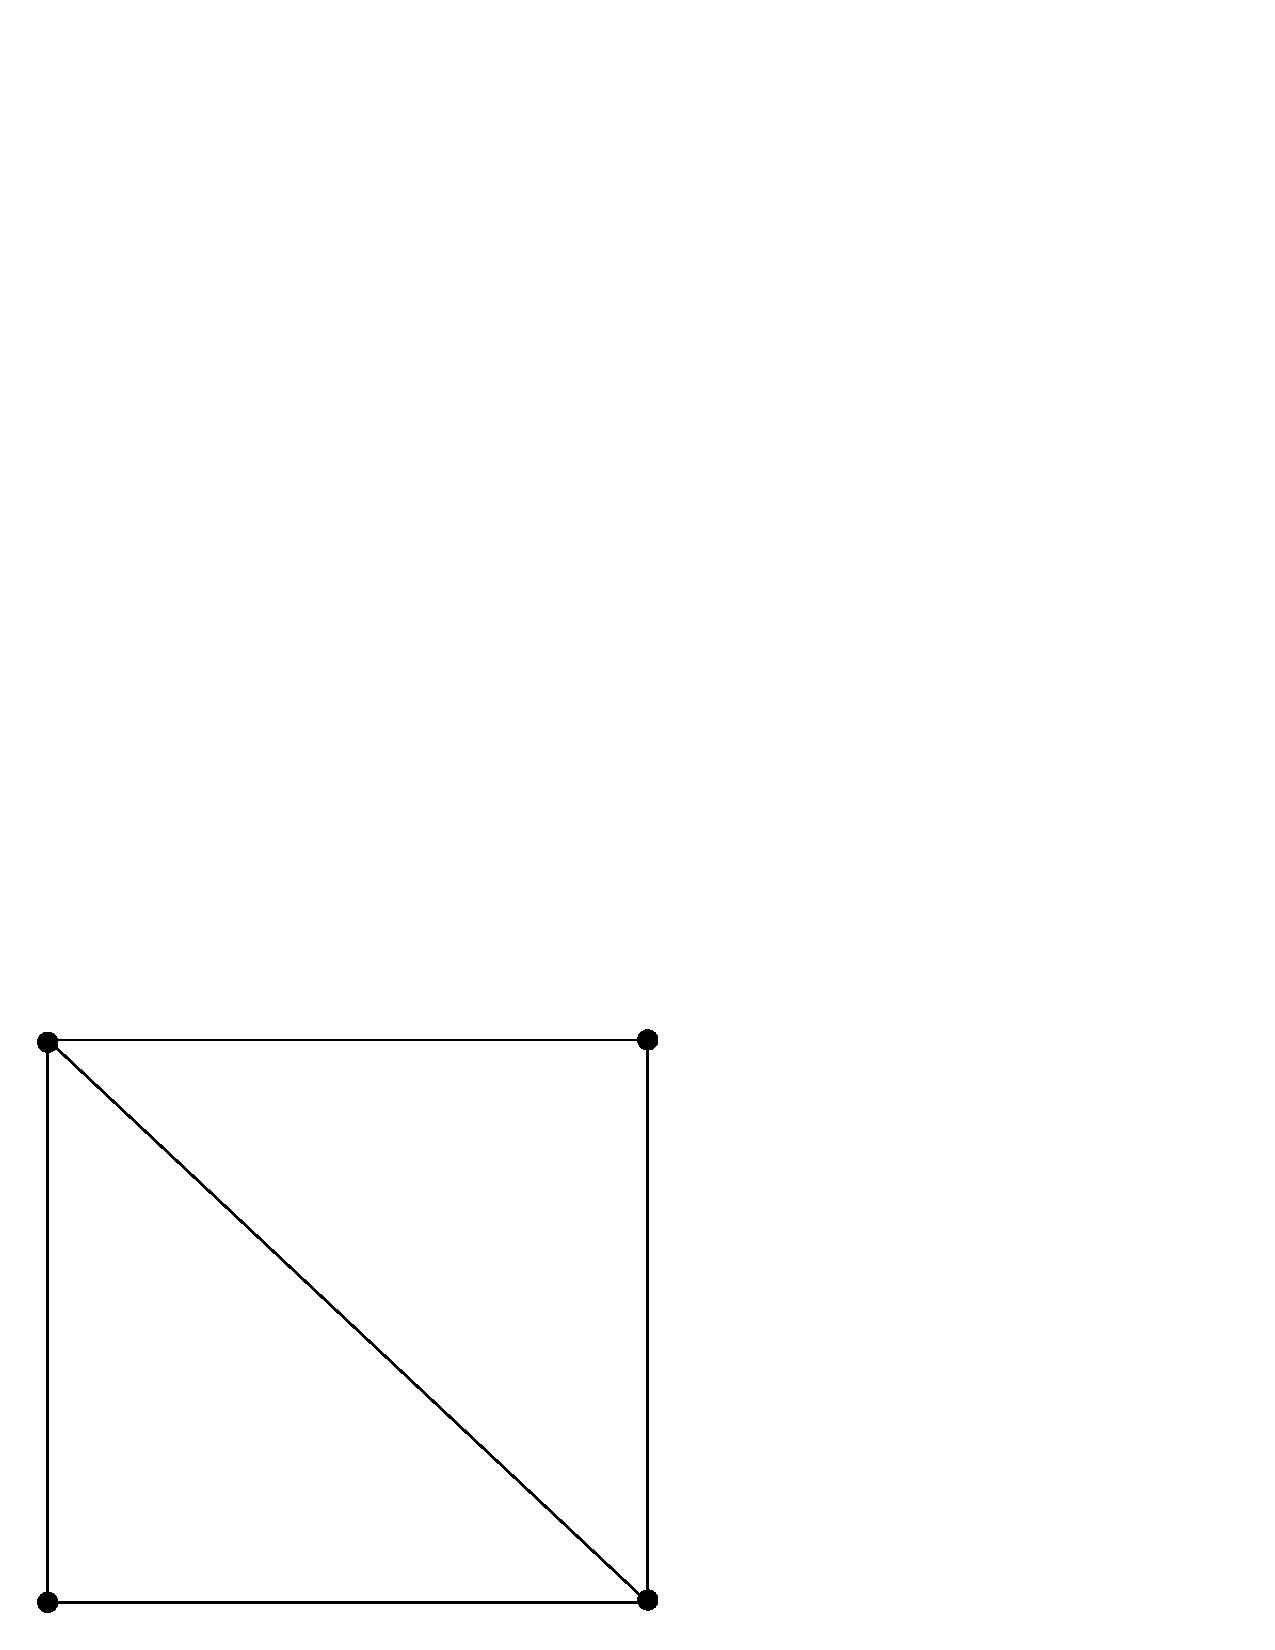
\includegraphics[width=0.3\textwidth]{./example}
\caption{One example}\label{ex}
\label{fig:example}
\end{figure}
\end{enumerate}

\end{document}	
